\documentclass{article}
\usepackage[utf8]{inputenc}
\usepackage[spanish]{babel}
\usepackage{float}
\usepackage{graphicx}
\usepackage{geometry}
\geometry{a4paper, margin=2.5cm}
\usepackage{pdfpages}

\begin{document}

\includepdf[pages=-]{caratula.pdf} % Inserta la carátula como primera página

\section*{2. Algoritmos de generación de reglas de clasificación: ZeroR, OneR, Prism}

\textbf{a) A partir de los datos del archivo \textit{Globos.xlsx} determine, utilizando los métodos \textbf{ZeroR y} \textbf{OneR,} el conjunto de reglas de clasificación que permita predecir si un globo dado permanecerá inflado o no (atributo \textit{Inflado?}).}

\vspace{0.5cm}

A continuación, se presenta la tabla de datos que se utilizará en todos los incisos:

\begin{table}[H]
    \centering
    \renewcommand{\arraystretch}{1.2}
    \begin{tabular}{|c|c|c|c|c|c|}
        \hline
        \textbf{Orden} & \textbf{Color} & \textbf{Volumen} & \textbf{Estira} & \textbf{Edad} & \textbf{Resultado} \\ \hline
        0 & Amarillo & Chico & Si & Adulto & Inflado \\ \hline
        1 & Amarillo & Chico & Si & Niño & Inflado \\ \hline
        2 & Amarillo & Grande & Si & Adulto & Inflado \\ \hline
        3 & Amarillo & Grande & Si & Niño & Inflado \\ \hline
        4 & Rojo & Chico & Si & Adulto & Inflado \\ \hline
        5 & Rojo & Grande & Si & Adulto & Inflado \\ \hline
        6 & Amarillo & Mediano & No & Adulto & No Inflado \\ \hline
        7 & Amarillo & Chico & No & Niño & No Inflado \\ \hline
        8 & Amarillo & Mediano & No & Adulto & No Inflado \\ \hline
        9 & Amarillo & Mediano & No & Niño & No Inflado \\ \hline
        10 & Rojo & Chico & Si & Niño & No Inflado \\ \hline
        11 & Rojo & Mediano & No & Adulto & No Inflado \\ \hline
        12 & Rojo & Mediano & No & Niño & No Inflado \\ \hline
        13 & Rojo & Grande & Si & Niño & No Inflado \\ \hline
        14 & Rojo & Grande & No & Adulto & No Inflado \\ \hline
        15 & Rojo & Grande & No & Niño & No Inflado \\ \hline
    \end{tabular}
    \caption{Dataset Globos.xlsx}
\end{table}

\vspace{0.5cm}

Dado que la resolución de este ejercicio requiere un desarrollo exhaustivo, los cálculos de las tasas de acierto y la determinación empírica de las reglas se han realizado de forma manual. Todo el procedimiento detallado paso a paso se encuentra adjunto en la sección de \textbf{Anexo} al final de este documento, a través de las capturas fotográficas de la resolución en papel.

A continuación, se presentan de forma resumida las tablas con los resultados finales obtenidos de dicho análisis.

\subsection*{Resumen de Reglas Obtenidas}

\begin{table}[H]
    \centering
    \renewcommand{\arraystretch}{1.5}
    \begin{tabular}{|l|p{4cm}|p{4cm}|p{4cm}|}
        \hline
        & \textbf{ZeroR} & \textbf{OneR} & \textbf{PRISM} \\ \hline
        \textbf{Reglas} 
        % Escribe aquí las reglas de ZeroR
        & Si(todo)entoces Resultado=No Inflado
        % Escribe aquí las reglas de OneR
        & Si(Estira)entonces Resultado=Inflado
        % Escribe aquí las reglas de PRISM
        \\ \hline
    \end{tabular}
    \caption{Comparativa de las reglas generadas por cada algoritmo.}
\end{table}

\subsection*{Análisis del Algoritmo OneR}

La siguiente tabla refleja el desglose de errores (o tasa de acierto) para cada posible regla derivada de cada atributo analizado.

\begin{table}[H]
    \centering
    \renewcommand{\arraystretch}{1.2}
    \begin{tabular}{|l|c|}
        \hline
        \textbf{Regla} & \textbf{Error} \\ \hline
        Si Color = Amarillo $\rightarrow$ Inflado (o No Inflado) & 4/8 \\ \hline
        Si Color = Rojo $\rightarrow$ No Inflado & 2/8 \\ \hline
        Si Volumen = Chico $\rightarrow$ Inflado & 2/5 \\ \hline
        Si Volumen = Mediano $\rightarrow$ No Inflado & 0/5 \\ \hline
        Si Volumen = Grande $\rightarrow$ Inflado (o No Inflado) & 3/6 \\ \hline
        Si Estira = Si $\rightarrow$ Inflado & 2/8 \\ \hline
        Si Estira = No $\rightarrow$ No Inflado & 0/8 \\ \hline
        Si Edad = Adulto $\rightarrow$ Inflado (o No Inflado) & 4/8 \\ \hline
        Si Edad = Niño $\rightarrow$ No Inflado & 2/8 \\ \hline
    \end{tabular}
    \caption{Tasas de error para cada regla posible (OneR).}
\end{table}

\vspace{0.3cm}
Finalmente, se detalla el error total asociado a cada atributo en su conjunto, lo cual permite determinar qué atributo se elige como discriminador principal:

\begin{table}[H]
    \centering
    \renewcommand{\arraystretch}{1.2}
    \begin{tabular}{|l|c|}
        \hline
        \textbf{Atributo} & \textbf{Error Total} \\ \hline
        Color & 6/16 \\ \hline
        Volumen & 5/16 \\ \hline
        Estira & 2/16 \\ \hline
        Edad & 6/16 \\ \hline
    \end{tabular}
    \caption{Error total calculado para cada atributo.}
\end{table}

\clearpage % Salto de página para que el anexo empiece en hoja nueva

\section*{Anexo: Resoluciones Manuales}

En esta sección se adjuntan las fotografías con el detalle de los cálculos realizados a mano para la obtención de las reglas y los errores (ZeroR, OneR y PRISM).

\subsection*{Ejercicio 2.a - ZeroR y OneR}

\begin{figure}[H]
    \centering
    % Descomenta y ajusta el nombre del archivo de la foto
    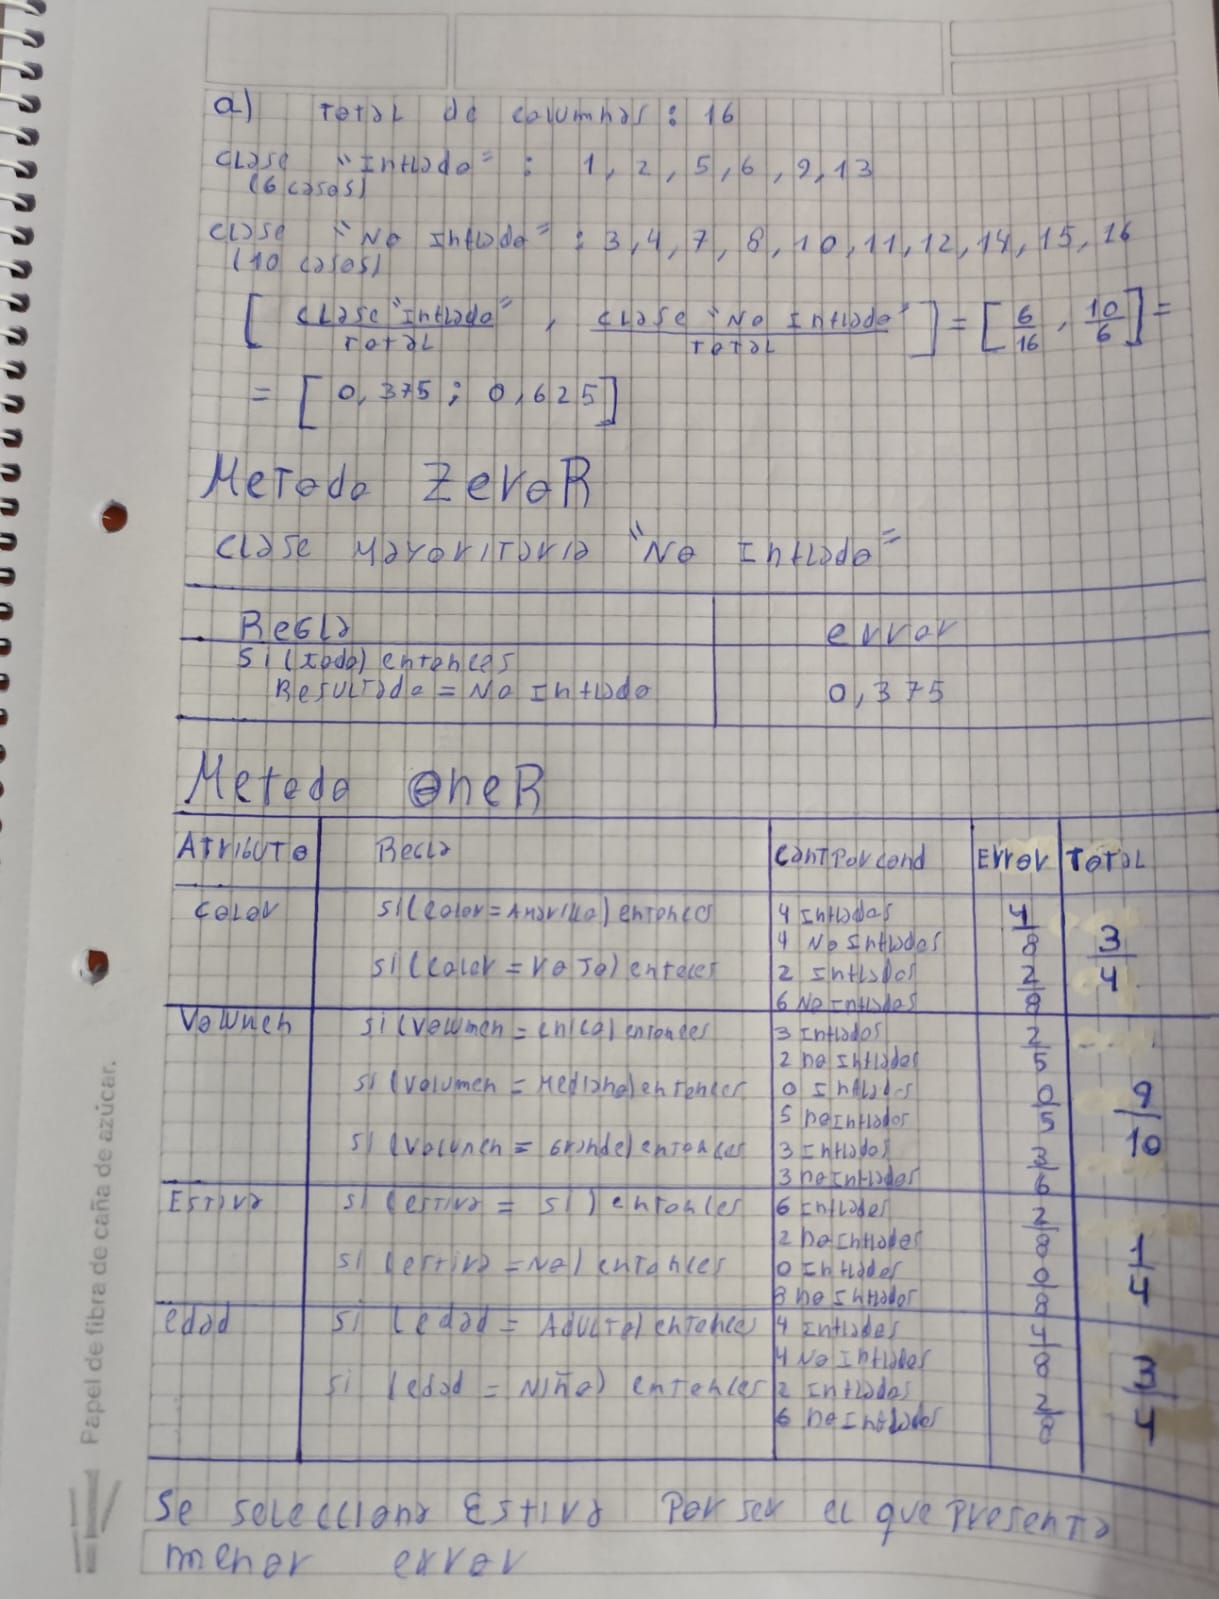
\includegraphics[width=0.8\textwidth]{EjercicioA.jpeg}
    \caption{Cálculos manuales: Resolución de ZeroR (Inciso a)}
\end{figure}

\begin{figure}[H]
    \centering
    % Descomenta y ajusta el nombre del archivo de la foto
    % \includegraphics[width=0.8\textwidth]{imagenes/resolucion_oner.jpg}
    \caption{Cálculos manuales: Cálculos de tasas de error para OneR (Inciso a)}
\end{figure}

\begin{figure}[H]
    \centering
    % Descomenta y ajusta el nombre del archivo de la foto
    % \includegraphics[width=0.8\textwidth]{imagenes/resolucion_prism.jpg}
    \caption{Cálculos manuales: Algoritmo PRISM}
\end{figure}

\end{document}